% Set page size and margins
\usepackage[
  a4paper,
  top=2.43cm,
  bottom=3cm,
  left=1.5cm,
  right=1.5cm,
  marginparwidth=1.75cm,
  footskip=2.05cm,
]{geometry}

% General language packages
\usepackage[T1]{fontenc}
\usepackage{fontspec}
\defaultfontfeatures{Mapping=tex-text}

% Useful packages
\usepackage[export]{adjustbox}
\usepackage{amsmath}
\usepackage{array}
\usepackage{caption}
\usepackage[strict]{changepage}
\usepackage{enumitem}
\usepackage{etoolbox}
\usepackage{float}
\usepackage{fullwidth}
\usepackage{graphicx, trimclip}
\usepackage[colorlinks=true, allcolors=blue]{hyperref}
\usepackage{hyperref}
\usepackage[noautomatic, nonewpage]{imakeidx}
\usepackage{multicol}
\usepackage{multirow}
\usepackage[super]{nth}
\usepackage{outlines}
\usepackage{paracol}
\usepackage[section]{placeins}
\usepackage{setspace}
\usepackage{stfloats}
\usepackage{subcaption}
\usepackage[usetransparent=false]{svg}
\usepackage{tabularx}
\usepackage[subfigure]{tocloft}
\usepackage{tikz}
\usepackage{titlesec}
\usepackage{transparent}
\usepackage{verbatim}
\usepackage{varwidth}
\usepackage{wrapfig}
\usepackage[most]{tcolorbox}
\usepackage{catchfile}
\usepackage{xstring}
\usepackage{soul}
\usepackage{xifthen}
\usepackage{xparse}

\usepackage{tocloft}
\renewcommand{\cftsubsecpagefont}{\bfseries}

\usepackage[hang, symbol, perpage]{footmisc}
\renewcommand{\footnotemargin}{1em}

\newtcolorbox{scaledfigure}[1][]{height fill, space to=\myspace,#1}
\hypersetup{
  colorlinks=true,
  linkcolor=goldenbrown,
  filecolor=magenta,
  urlcolor=cyan,
  pdftitle={Heroes of Might \& Magic III Fan-Made Draft Scenarios},
  pdfpagemode=UseNone,
}
% Set the default spacing between paragraphs. Remove indentation.
\usepackage[skip=6pt, indent=0pt]{parskip}
\setstretch{1}

% Default margins for itemize lists
\setlist[itemize,2]{leftmargin=15pt, label=$\triangleright$}
\setlist[enumerate,2]{leftmargin=15pt}

% Get version from env
% \getenv{variable_name} just prints the value
% \getenv[\macro]{variable_name} stores the value in \macro for reusability
\newcommand{\getenv}[2][]{%
  \CatchFileEdef{\value}{"|echo \$#2"}{\endlinechar=-1}%
  \if\relax\detokenize{#1}\relax\value\else\let#1\value\fi}

% Add dots to the table of contents
\renewcommand{\cftsecleader}{\cftdotfill{\cftsecdotsep}}
\renewcommand\cftsecdotsep{\cftdot}
\renewcommand\cftsubsecdotsep{\cftdot}

\captionsetup[figure]{labelformat=empty}
\captionsetup[subfigure]{labelformat=empty, singlelinecheck=off, justification=centering}
\usetikzlibrary{shadows, shadows.blur, patterns, calc, backgrounds, arrows.meta, babel}

\setlength{\columnsep}{1cm}
\newtoggle{printable}
\newtoggle{noartbackground}
\newtoggle{githubbuild}

% Variables
\def\_assets{assets}

\def\art{\_assets/art}
\def\cards{\_assets/cards}
\def\examples{\_assets/examples}
\def\images{\_assets/images}
\def\layout{\_assets/layout}
\def\maps{\_assets/maps}
\def\skills{\_assets/skills}
\def\spells{\_assets/spells}
\def\svgs{\_assets/glyphs}
\def\notes_svgs{\svgs/for-notes}
\def\tables{\_assets/tables}
\def\qr{\_assets/qr-codes}

\def\repourl{https://github.com/qwrtln/Homm3BG-mission-book}

\newcommand{\svg}[2][10]{%
  {\raisebox{-0.15\height}{\includesvg[height=#1px]{\svgs/\detokenize{#2}.svg}}}%
}%

\newcommand{\bronze}[1][10]{%
  \leavevmode\hbox{\raisebox{-0.1\height}{\includesvg[height=#1px]{\iftoggle{noartbackground}{\svgs/bronze-mono.svg}{\svgs/bronze.svg}}}}%
}%

\newcommand{\silver}[1][10]{%
  \leavevmode\hbox{\raisebox{-0.1\height}{\includesvg[height=#1px]{\iftoggle{noartbackground}{\svgs/silver-mono.svg}{\svgs/silver.svg}}}}%
}%

\newcommand{\golden}[1][10]{%
  \leavevmode\hbox{\raisebox{-0.1\height}{\includesvg[height=#1px]{\iftoggle{noartbackground}{\svgs/golden-mono.svg}{\svgs/golden.svg}}}}%
}%

\newcommand{\azure}[1][10]{%
  \leavevmode\hbox{\raisebox{-0.1\height}{\includesvg[height=#1px]{\iftoggle{noartbackground}{\svgs/azure-mono.svg}{\svgs/azure.svg}}}}%
}%

\newcommand{\svgeven}[2][10]{%
  \includesvg[height=#1px]{\svgs/\detokenize{#2}.svg}%
}%

\renewcommand{\labelitemi}{
  \begin{tikzpicture}
    \node (listdot) [circle, inner sep=-3] {
\includegraphics[width=1em, valign=c]{\layout/listdot.png}};
  \end{tikzpicture}
}

% Colors
\definecolor{amber}{rgb}{1.0, 0.49, 0.0}
\definecolor{antiquewhite}{rgb}{0.98, 0.92, 0.84}
\definecolor{arylideyellow}{rgb}{0.96, 0.89, 0.58}
\definecolor{bistre}{rgb}{0.24, 0.17, 0.12}
\definecolor{cadmiumgreen}{rgb}{0.0, 0.42, 0.24}
\definecolor{camel}{rgb}{0.76, 0.6, 0.42}
\definecolor{cobalt}{rgb}{0.0, 0.28, 0.67}
\definecolor{darkcandyapplered}{rgb}{0.64, 0.0, 0.0}
\definecolor{darkyellow}{RGB}{204, 154, 0}
\definecolor{deepskyblue}{rgb}{0.0, 0.75, 1.0}
\definecolor{goldenbrown}{rgb}{0.6, 0.4, 0.08}

% Command to frame images
\newcommand\framedimage[2][]{%
  \begin{tikzpicture}
    \draw (0, 0) node[inner sep=0] {\makebox[#1][c]{\includegraphics[width=#1]{#2}}};
    \draw [bordermidyellow, thick] ([xshift=+1pt, yshift=-1pt] current bounding box.north west) rectangle ([xshift=-1pt, yshift=1pt] current bounding box.south east);
    \draw [borderoutyellow, thick] (current bounding box.north west) rectangle (current bounding box.south east);
    \draw [borderinyellow, thick] ([xshift=+3pt, yshift=-3pt] current bounding box.north west) rectangle ([xshift=-3pt, yshift=3pt] current bounding box.south east);
  \end{tikzpicture}}
% End of drop frame definition

\titleformat{\section}
{\huge}
{\filright
\footnotesize
\enspace SECTION \thesection\enspace}
{8pt}
{\Huge\bfseries\filcenter\uppercase}

\newfontfamily{\liberation}{LiberationSerif}
[
  Path = ./assets/fonts/,
  Extension = .ttf,
  UprightFont = *-Regular,
  ItalicFont = *-Italic,
  BoldFont = *-Bold,
  BoldItalicFont = *-BoldItalic
]

\newcommand{\sectionheadertext}[2][antiquewhite]{
  \iftoggle{noartbackground}{}{\color{#1}}\MakeUppercase{\textbf{\liberation #2}}
}

%Create section heading with graphics. Argument one is heading name, argument two is picture to use on the left.
\newcommand{\addsection}[2]{
  \vspace*{-5.72em}
  \hspace*{-1.3em}
  \makebox[0pt][l]{
  \raisebox{-\totalheight}[0pt][7pt]{
      \begin{tikzpicture}
        \iftoggle{noartbackground}{
          \draw (0, 0) node[inner sep=0] (header){\makebox[1.015\textwidth][c]{
\includegraphics[width=1.055\linewidth, height=0.24\linewidth]{\layout/section_heading_monochrome.png}}};
        }{
          \draw (0, 0) node[inner sep=0] (header){\makebox[1.015\textwidth][c]{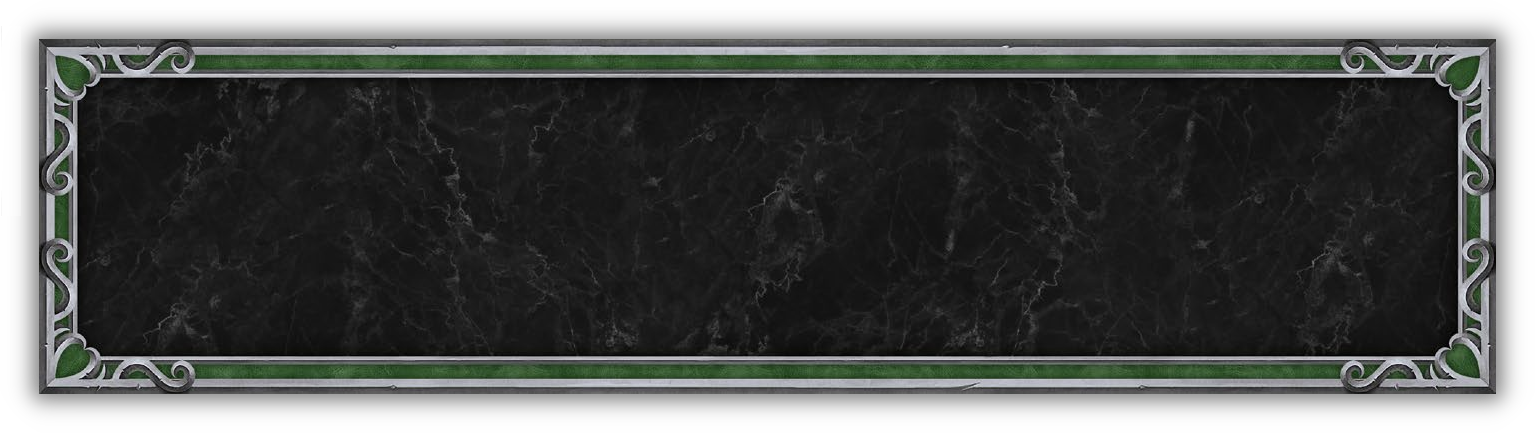
\includegraphics[width=1.055\linewidth, height=0.24\linewidth]{\layout/section_heading.png}}};
        }
        \draw (-6.7, 0) node {\includegraphics[width=0.135\textwidth]{#2}};
      \end{tikzpicture}
    }
  }
  \begin{fullwidth}[leftmargin=0.21\textwidth]
    \begin{center}
      \vspace{1em}
      \vspace{\lang_header_adjustment}
      \section*{\sectionheadertext{#1}}
      \cleardoublepage\phantomsection\addcontentsline{toc}{section}{\protect\numberline{}#1}
      \pagetarget{#1}{}
    \end{center}
  \end{fullwidth}
  \vspace{1.75em}
  \vspace{\lang_header_adjustment}
}
%End of create section heading.

% Add title page for Scenario type
\newcommand{\addscenariogroup}[2]{
  \thispagestyle{empty}
  \cleardoublepage\phantomsection\addcontentsline{toc}{section}{\protect\numberline{}#1}
  \iftoggle{noartbackground}{}{
    \AddToHookNext{shipout/background}{%
      \put (0in,-\paperheight){
\includegraphics[width=\paperwidth,height=\paperheight]{\layout/tausta.png}}%
    }
  }
  \begin{tikzpicture}[remember picture, overlay, inner sep=10pt]
    \iftoggle{noartbackground}{}{
      \node(cover)[anchor=center] at (current page.center) {
        \includegraphics[height=\paperheight, keepaspectratio]{#2}
      };
    }
    \node(heading)[anchor=center] at (current page.center) {
      
\includegraphics[width=\linewidth, keepaspectratio]{\layout/grouping_heading.png}
    };
    \node(title)[minimum width = \paperwidth, anchor=center] at (current page.center) {
      \huge\sectionheadertext[bistre]{#1}
    };
  \end{tikzpicture}
}

\newcommand\addheadershadow[2][]{
    % #1: Optional aditional tikz options
    % #2: Name of the node to "decorate"
    \begin{pgfonlayer}{background}
        \path[
           rounded corners=1pt,
           blur shadow={shadow xshift=0pt,
           shadow yshift=0pt,
           shadow blur steps=10,
           shadow blur radius=6pt}, #1]
            ($(#2.north west)+( 0.6pt,0)$) --
            ($(#2.south west)+( 0.6pt,0)$) --
            ($(#2.south east)+(-0.6pt,0)$) --
            ($(#2.north east)+(-0.6pt,0)$) --
        cycle;
        \path[rounded corners,
           blur shadow={shadow xshift=0pt,
           shadow yshift=0pt,
           shadow blur steps=10,
           shadow blur radius=6pt}, #1]
            ($(#2.north west)+(-1.3pt,-3pt)$) --
            ($(#2.south west)+(-1.3pt, 3pt)$) --
            ($(#2.south east)+( 1.3pt, 3pt)$) --
            ($(#2.north east)+( 1.3pt,-3pt)$) --
            cycle;
    \end{pgfonlayer}
}

% Four mandatory params
% - [optional] set to "subsection" or any other Level if you want to have this as a subsection in TOC
% - Lines of Campaign Name (1-2 according to the name length)
% - Campaign Name
% - Scenario Name
% - Icon
%
% TODO: possibly replace the whole \addsection with this
\newcommand{\addscenariosection}[5][section]{
  \sodef\sotitle{}{0.2em}{0.6em}{1.2em}
  \def\oneliner{\equal{#2}{1}}

  \vspace*{-5.72em}
  \hspace*{-1.3em}
  \makebox[0pt][l]{
  \raisebox{-\totalheight}[0pt][7pt]{
    \ifthenelse{\oneliner}{\def\yscale{1}}{\def\yscale{1.3}}
      \begin{tikzpicture}
        \iftoggle{noartbackground}{
          \draw (0, 0) node[inner sep=0, yscale=\yscale] (header){\makebox[1.015\textwidth][c]{
\includegraphics[width=1.055\linewidth, height=0.24\linewidth]{\layout/section_heading_monochrome.png}}};
        }{
          \draw (0, 0) node[inner sep=0, yscale=\yscale] (header){\makebox[1.015\textwidth][c]{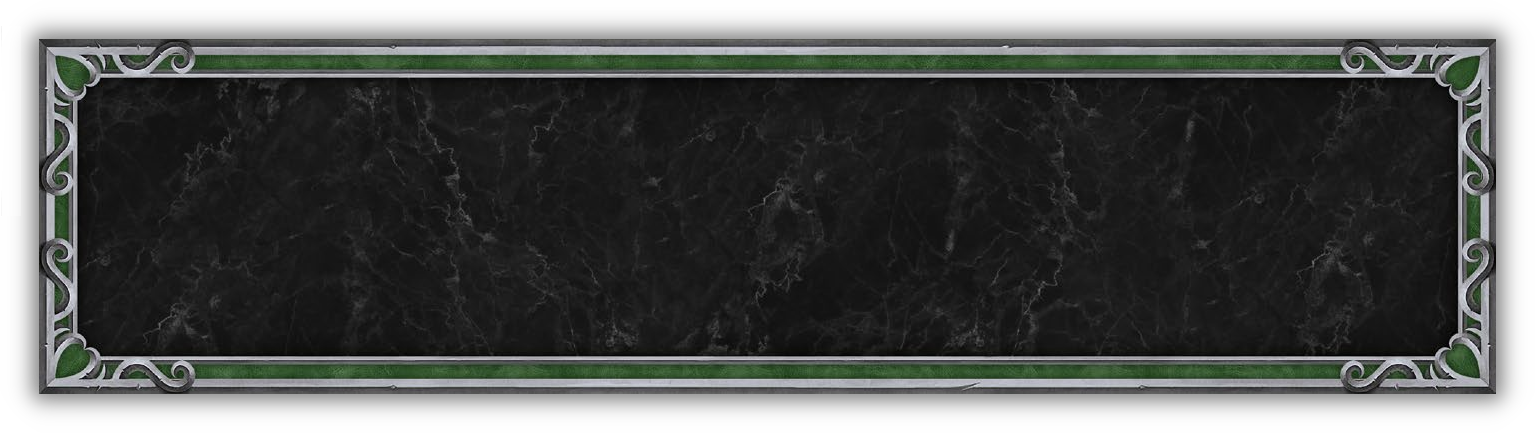
\includegraphics[width=1.055\linewidth, height=0.24\linewidth]{\layout/section_heading.png}}};
        }
        \draw (-6.7, 0) node {\includegraphics[width=0.135\textwidth]{#5}};
      \end{tikzpicture}
    }
  }
  \begin{fullwidth}[leftmargin=0.21\textwidth]
    \begin{center}
      \vspace{\lang_header_adjustment}
      \vspace{-12pt}
      \section*{\sectionheadertext{\small{\sotitle{#3}}}}
      \vspace{\lang_header_adjustment}
      \vspace{-10pt}
      \section*{\sectionheadertext{#4}}
      \ifthenelse{\oneliner}{}{\vspace{14pt}}
      \cleardoublepage\phantomsection\addcontentsline{toc}{#1}{\protect\numberline{} {} {} {} {}#4}
      \pagetarget{#4}{}
    \end{center}
  \end{fullwidth}
  \ifthenelse{\oneliner}{\vspace{1.75em}}{\vspace{0.75em}}
  \vspace{\lang_header_adjustment}
}

% Apply language-specific subsection spacings if defined
\ifdefined\subsectionspacing
  \subsectionspacing{}
\fi

\newcommand\picdims[4][]{%
  \setbox0=\hbox{\includegraphics[#1]{#4}}%
  \clipbox{.5\dimexpr\wd0-#2\relax{} %
    .5\dimexpr\ht0-#3\relax{} %
    .5\dimexpr\wd0-#2\relax{} %
    .5\dimexpr\ht0-#3\relax}{\includegraphics[#1]{#4}}}

\tikzset{
  thick/.style=      {line width=1.3pt},
  very thick/.style= {line width=1.7pt},
  ultra thick/.style={line width=2.2pt}
}

\definecolor{borderoutyellow}{HTML}{DBCA86}
\definecolor{borderinyellow}{HTML}{B09E69}
\definecolor{bordermidyellow}{HTML}{6f6749}
% Create note box
\newcommand{\notefont}[0]{\liberation\selectfont}
\newcommand{\note}[2]{
  \begin{tikzpicture}
    \draw (0, 0) node[inner sep=0] {\makebox[\linewidth][c]{\picdims[width=\linewidth]{\linewidth}{#1\baselineskip}{\layout/table-background.jpg}}};
    \draw [borderoutyellow, very thick] (current bounding box.north west) rectangle (current bounding box.south east);
    \draw [borderinyellow, thick] ([xshift=+2.8pt, yshift=-2.8pt] current bounding box.north west) rectangle ([xshift=-2.8pt, yshift=2.8pt] current bounding box.south east);
    \node at (current bounding box.center) {
      \begin{varwidth}{0.85\linewidth}
      \notefont{
        \color{arylideyellow}
        \hypersetup{linkcolor=amber}
        #2
        \hypersetup{linkcolor=goldenbrown}
      }
      \end{varwidth}
    };
    \begin{pgfonlayer}{background}
      \begin{scope}[blend mode=multiply]
        \draw [shade, blur shadow={shadow opacity=15}] (current bounding box.north west) rectangle (current bounding box.south east);
      \end{scope}
    \end{pgfonlayer}
  \end{tikzpicture}
}

% Create Heroes-styled framed canvas for a table. Accepts three arguments:
% 1) [Optional] Drop shadow description. Use [] as the first arg to delete it.
% 2) Height specified in verses (lines of text)
% 3) Table contents like title and tabularx environment
\newcommand{\hommtable}[3][shade, blur shadow={shadow opacity=15}]{
  \begin{tikzpicture}
    \iftoggle{noartbackground}{
      \node[inner sep=0, minimum width=\linewidth, minimum height=#2\baselineskip] at (0,0) {};
    }{
      \draw (0, 0) node[inner sep=0] {\makebox[\linewidth][c]{\picdims[width=\linewidth]{\linewidth}{#2\baselineskip}{\layout/table-background.jpg}}};
    }
    \draw [bordermidyellow, thick] ([xshift=+1pt, yshift=-1pt] current bounding box.north west) rectangle ([xshift=-1pt, yshift=1pt] current bounding box.south east);
    \draw [borderoutyellow, thick] (current bounding box.north west) rectangle (current bounding box.south east);
    \draw [borderinyellow, thick] ([xshift=+3pt, yshift=-3pt] current bounding box.north west) rectangle ([xshift=-3pt, yshift=3pt] current bounding box.south east);
    \node at (current bounding box.center) {
      \begin{varwidth}{0.95\linewidth}
      \notefont{
        \bgroup
        \iftoggle{noartbackground}{}{
          \color{arylideyellow}
          \hypersetup{linkcolor=amber}
        }
        \setlength{\tabcolsep}{0.3em}
        #3
        \egroup
      }
      \end{varwidth}
    };
    \begin{pgfonlayer}{background}
      \begin{scope}[blend mode=multiply]
        \draw [#1] (current bounding box.north west) rectangle (current bounding box.south east);
      \end{scope}
    \end{pgfonlayer}
  \end{tikzpicture}
}
% End of Heroes-styled canvas definition.

% Redefinition of the table for mutlicol enviromnents
\newcommand{\hommtablemulticol}[3][shade, blur shadow={shadow opacity=15}]{
  \begin{tikzpicture}
    \iftoggle{noartbackground}{
      \node[inner sep=0, minimum width=\linewidth, minimum height=#2\baselineskip] at (0,0) {};
    }{
      \draw (0, 0) node[inner sep=0] {\makebox[\linewidth-3pt][c]{\picdims[width=\linewidth-3pt]{\linewidth-3pt}{#2\baselineskip}{\layout/table-background-multicol.jpg}}};
    }
    \draw [bordermidyellow, thick] ([xshift=+1pt, yshift=-1pt] current bounding box.north west) rectangle ([xshift=-1pt, yshift=1pt] current bounding box.south east);
    \draw [borderoutyellow, thick] (current bounding box.north west) rectangle (current bounding box.south east);
    \draw [borderinyellow, thick] ([xshift=+3pt, yshift=-3pt] current bounding box.north west) rectangle ([xshift=-3pt, yshift=3pt] current bounding box.south east);
    \node at (current bounding box.center) {
      \begin{varwidth}{\linewidth-3pt}
      \notefont{
        \bgroup
        \iftoggle{noartbackground}{}{
          \color{arylideyellow}
          \hypersetup{linkcolor=amber}
        }
        \setlength{\tabcolsep}{0.3em}
        #3
        \egroup
      }
      \end{varwidth}
    };
    \begin{pgfonlayer}{background}
      \begin{scope}[blend mode=multiply]
        \draw [#1] (current bounding box.north west) rectangle (current bounding box.south east);
      \end{scope}
    \end{pgfonlayer}
  \end{tikzpicture}
}

\definecolor{darkcellborder}{HTML}{634831}
\definecolor{darkcellbg}{HTML}{20160C}

\newcommand{\darkcell}[2][0.9]{
  \begin{tikzpicture}
    \filldraw[line width=1.0pt, fill=darkcellbg, fill opacity=0.5, draw=darkcellborder] (0, 0) rectangle (\linewidth, #1);
    \node[text width=\linewidth, align=center] at (current bounding box.center) {\textbf{#2}};
  \end{tikzpicture}
}

\newcommand{\darkcellleft}[2][0.9]{
  \begin{tikzpicture}
    \filldraw[line width=1.0pt, fill=darkcellbg, fill opacity=0.5, draw=darkcellborder] (0, 0) rectangle (\linewidth, #1);

    \node[text width=\linewidth, align=left] at (current bounding box.center) {
      \leftskip=0.4em
      \rightskip=0pt plus 1fil
      \textbf{#2}\\
    };
  \end{tikzpicture}
}

\definecolor{lightcellborder}{HTML}{77543e}
\definecolor{lightcellbg}{HTML}{20160C}

\newcommand{\lightcell}[2][0.9]{
  \begin{tikzpicture}
    \filldraw[line width=1.0pt, fill=\iftoggle{noartbackground}{white}{lightcellbg}, fill opacity=0.25, draw=lightcellbg, fill opacity=0.25, draw=lightcellborder] (0, 0) rectangle (\linewidth, #1);
    \node[text width=\linewidth, align=center] at (current bounding box.center) {\iftoggle{noartbackground}{}{\color{white}}#2};
  \end{tikzpicture}
}

\newcommand{\lightcellleft}[2][0.9]{
  \begin{tikzpicture}
    \filldraw[line width=1.0pt, fill=\iftoggle{noartbackground}{white}{lightcellbg}, fill opacity=0.25, draw=lightcellbg, fill opacity=0.25, draw=lightcellborder] (0, 0) rectangle (\linewidth, #1);
    \node[text width=\linewidth, align=left] at (current bounding box.center) {
      \iftoggle{noartbackground}{}{\color{white}}
      \leftskip=0.4em
      \rightskip=0pt plus 1fil
      #2\\
    };
  \end{tikzpicture}
}

% Commands to be used for automation generating printable version
\newcommand{\pagetarget}[2]{\label{#1}\hypertarget{#1}{#2}}
\newcommand{\pagelink}[2]{\hyperlink{#1}{#2}\iftoggle{printable}{ \textmd{(\pageshorthand\,\pageref{#1})}}{}}

% Command for overlay circled text
\definecolor{goblin}{HTML}{3b7c33}
\newcommand\encircle[1]{%
  \tikz[baseline=(X.base)]
  \node (X) [draw=white, shape=circle, inner sep=0, fill=goblin, text=white, blur shadow={shadow blur steps=5}] {\strut \textbf{#1}};%
}

% Background
\AddToHook{shipout/background}{%
  \iftoggle{noartbackground}{}{
    \put (0in,-\paperheight){
\includegraphics[width=\paperwidth,height=\paperheight]{\layout/tausta.png}}
  }
  \put (0in,-\paperheight){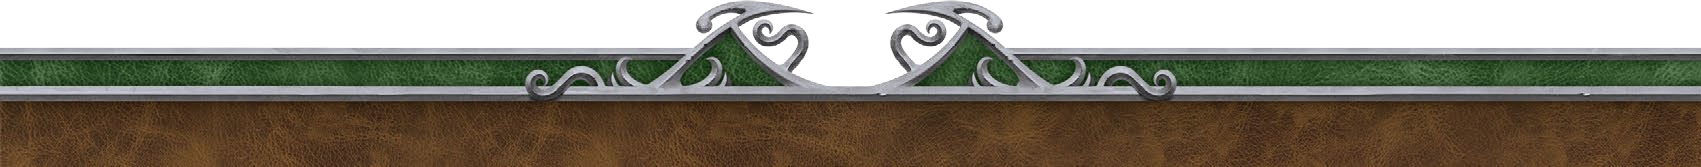
\includegraphics[width=\paperwidth,height=0.05\paperheight]{\layout/bottom.png}}
}

\begin{document}

\addsection{Dice Stacks Mod}{\images/luck.png}

\begin{multicols*}{2}
    \subsection*{Preparation}
    
    This modification will require additional content:
    \begin{itemize}
        \item Standard six-sided dice: minimum 4, around 8 is usually enough.
        \item Something to represent \textbf{Quantity Tokens} to put on the Unit Cards. The game's Gold Tokens may serve this role.
    \end{itemize}
    
    \subsection*{Quantity Tokens}
    
    The "Few" and "Pack" sides of Faction Units do not represent the stack size anymore. Instead, all Unit Cards may have any number of \textbf{Quantity Tokens} on them. Every Quantity Token:
    \begin{itemize}
        \item increases number of dice rolled when attacking by one (see \textit{Damage calculation});
        \item may be removed to reduce damage taken from any source by number depending on the Unit's tier.
    \end{itemize} 
    
    \medskip
    
    \note{5}{
        \textit{Reducing \svg{health_points-note} to 0} is treated as taking damage equal to current number of \svg{health_points-note} and may be reduced by removing Quantityu Tokens accordingly.
    }
    
    When a Unit is destroyed, remove all Quantity Tokens from it.
    
    \textbf{Example} \textit{Alice's Gorgons have one Quantity Token and 3 Damage. They are struck by Lightning Bolt with 1 \svg{empower}. Alice removed the Quantity Token -- as Gorgons are of \svg{silver} tier, this reduces the damage by 2. The Gorgons takes 1 Damage and survives this otherwise fatal blow.}
    
    \subsection*{Upgrading Units}
    
    "Pack" side of the unit is now refered as \textbf{"Upgraded"} side. When "Upgraded" Unit \svg{health_points} are reduced to $0$, you do not flip the card -- the Unit is defeated and discarded from your Units Deck.
    
    Faction Units may be "Upgraded" even outside of your Unit Deck. They keep the "Upgrade" status when discarded. The recruitment cost of "Upgraded" Unit is equal to its printed \svg{reinforce} value. \textbf{It is not} summed with \svg{pay} value.
    
    \medskip
    
    \note{5}{
        You may voluntarily flip back "Upgraded" Faction Unit before recruitment, to pay the lower \svg{pay-note} price for it.
    }
    
    Flipping the unit card to "Upgraded" side is now called \textbf{Upgrading}. You may Upgrade one of your Faction Units by using Build Token (not Population Token) -- it does not have to be in your Unit Deck, but you must have a corresponding Dwelling in your Town. 
    
    Always when Upgrading a Unit in your Unit Deck, you keep all Quantity Tokens on this Unit, but must pay the difference between \svg{reinforce} and \svg{pay}.
    
    \textbf{Example} \textit{During his Turn, Bobs flips the Buld Token and upgrades Gryffins in his Unit Deck paying 2~\svg{gold}. He cannot upgrade or build buildings anymore this Turn. He then flips the Population Token to Recruit Upgraded Marksmen which he had lost in previous Combat, what costs him 5~\svg{gold}.}
    
    \subsection*{Reinforcing Units}
    
    \textbf{Reinforcing} has now a different meaning: adding one \textbf{Quantity Token} to a Unit. The cost of Reinforcing is half of the Unit's base \svg{pay} cost, rounded down if it would be odd Quantity Token on this Unit, and rounded up otherwise.
    
    \medskip
    
    \note{3}{
        Upgrading a Unit does not increase its Reinforce cost -- it is stil half of the \svg{pay-note} value.
    }
    
    You do not need \textit{Citadel} to Reinforce Units anymore, but the number of times you may Recruit or Reinforce a Unit when using Population Token is now limited:
    \begin{itemize}
        \item you may freely Recruit or Reinforce any Unit once;
        \item for every Flagged \textbf{Settlement} not contributing to your Resource Income you may Recruit or Reinforce one Unit which was not yet Recruited or Reinforced during this Action.
        \item \textbf{Citadel} allows one more Recruitment or Reinforcement of any Unit, even it it was already Recruited or Reinforced.
    \end{itemize}
    
    \subsection*{Damage calculation}
    
    The table below shows how many six-sided Dice are assigned to a Unit according to its tier. Every \textbf{Quantity Token} increases this number by one.
    
    When a Unit attacks, instead of rolling Attack Dice, you rolls the assigned number of six-sided Dice. A sufficiently high result on a die is considered a hit and delivers one point of damage:
    \begin{itemize}
        \item "6" always hits, "1" always misses
        \item otherwise the minimum to-hit value is equal to $6 - \svg{attack} \text{ of the attacker} + \svg{defense} \text{ of the defender}$".
    \end{itemize}
    Additionally:
    \begin{itemize}
        \item every defender's \svg{defense} point exceeding attacker's \svg{attack} reduces damage by 1, but not below 0,
        \item every attacker's \svg{attack} point exceeding defender's $\svg{defense} + 4$ increases damage by 1, but not above the number of Dice.
    \end{itemize}
    
    The delivered damage may be then reduced by the defending Unit's owner by removing Quantity Tokens from the Unit. The damage reduction depends on defending Unit's tier -- consult the Table below. This is done before the damage is applied, so its possible to reduce damage which would otherwise defeat the Unit.
    
    \hommtablemulticol{13}{
        \centering
        \begin{tabularx}{0.96\linewidth}{p{0.12\linewidth}XX}
            \darkcell[1.2]{} & \darkcell[1.2]{Base Dice count} & \darkcell[1.2]{Damage reduction} \\
            \lightcell{\svg{bronze}} & \lightcell{2} & \lightcell{1} \\
            \lightcell{\svg{silver}} & \lightcell{3} & \lightcell{2} \\
            \lightcell{\svg{golden}} & \lightcell{4} & \lightcell{3} \\
            \lightcell{\svg{azure-note}} & \lightcell{5} & \lightcell{4} \\
        \end{tabularx}
    }
    
    \textbf{Example} \textit{Bob's Upgraded Pit Lords with 4 Quantity Tokens attack Alice's Black Dragons. Alice plays Defense Card. With Pit Lords' 5~\svg{attack} and Dragons' 4~\svg{defense} the value to-hit is 5. Bob rolls 6, 1, 4, 5, 3, 6, 2, what gives 3 Damage total.}
        
    \textit{Now it is time for Black Dragons' retaliation: The \svg{attack} and \svg{defense} is now 5, what would give to-hit value of 1, but "1" always misses anyway. However, because the difference is higher that 4, Dragons may add additional point of Damage. Alice rolls 1, 1, 4, 5, what gives the total Damage of 3. Even if no "1" would be rolled, the damage couldn't be higher than 4 -- the number of Dice.}
    
    \subsection*{M\&M Discard Reshuffle}
    
    If you are drawing Cards from your M\&M Deck and the Deck is empty, you stop drawing and \textbf{do not reshuffle} your Discard Pile and do not form a new M\&M Deck.
    
    Instead, the Deck is reformed at start of your Turn: between discarding Cards and drawing up to Hand Limit, you shuffle your Discard Pile and put it under the current M\&M Deck. 
    
    \subsection*{Drawing new Hand during Combat}
    
    When a Combat continues to the next Round: \begin{itemize}
        \item you first resolve all effects taking place at end of Combat Round (like discarding some \svg{ongoing} Cards),
        \item then you may discard any number of Cards - you don't need to go under Hand Limit,
        \item and after that \textbf{you draw Cards up to your Hand Limit}
    \end{itemize}
    
    \subsection*{Playing M\&M Cards}
    
    \textbf{Playing M\&M Cards is now more restricted}: you may play them in three situations: \begin{itemize}
        \item During Combat, according to the standard Rules, but you cannot receive Resources nor \svg{movement}.
        \item Outside Combat, immediately after gaining them to your Hand.
        \item At the beginning of your Turn, after initial drawing up to Hand Limit and before any Movement Action.
    \end{itemize}
    
    When a Card is played outside Combat, you may decide to delay Card's effect: you may resolve it later this Turn at any momend allowed by the Effect, \textbf{but not during Combat}. In other words, the played Card may be treated as it would have "\svg{ongoing} Once this Turn, outside Combat:" before the actual text.
    
    \note{6}{
        When delaying Artifact or Ability Card's effect, you still must choose which option you take option and spent \svg{expert} right after playing.
    }
    
    \textbf{Example 1} \textit{Alice just got Learning ability from Witch Hut. Seeing Tree of Knowledge ahead, she decides to play it and delay the Basic effect. Then moves her Hero to the Tree, and while leveling-up, resolves the Learing Effect gainig additional 1 \svg{experience}.}
    
    \textbf{Example 2} \textit{Second Round of Bob's Combat just started. He discard and draw Cards up to Hand Limit -- among others he sees Estate Ability. Playing it now would waste the Effect, as he cannot get Resources during Combat. The Combat finishes, but he still cannot play it, because he already moved Hero. He keeps the Card until his next Turn, where -- after discarding and drawing up to Hand Limit -- he may finally play the Ability and get his bounty.}
            
    \subsection*{Morale}
    
    While you have Negative Morale Token, \textbf{the hand limit during Combat is reduced by~1}.
    
    \textbf{You discard Morale Token} (both Positive and Negative) \textbf{at end of a Combat}. If the Morale was Positive, you may perform a Morale Action.
    
    \textbf{The penalty for second Negative Morale is changed}: every time you woud take a second Negative Morale Token:
    \begin{itemize}
        \item you discard one card from hand immediately
        \item the hand limit for your next turn's initial draw is reduced by 1 (the draws during Combat are not affected). Put a black cube on the current card limit icon of your Hero's Level Tracker as a reminder. 
    \end{itemize} 
    \textbf{The latter effect is cumulative}: if during same turn you again would take Negative Morale Token while still having one, you limit is again reduced and you put another black cube on Level Tracker. However, your limit could never drop below 3 cards.
    
    \textbf{Example} \textit{Alice's Main Hero has Level V, so her Hand Limit is 6, but she has a token. She moves her Hero to a guarded field with Warrior Tomb. The fight is fierce, and Alice starts her second Combat Round without Cards. She draws 5 Cards -- reduced Limit because of the Negative Morale Token. Still she defeats her opponents in the second Round, and discards the Negative Morale}
    
    \textit{She decides to visit the Tomb, getting 2 \svg{morale_negative}. She gets Negative Morale Token again, discard a Card, and place a black cube on the icon under V on her Level Tracker. One of the gained Artifacts happens to be Crest of Valor, which she plays immediately. She discards Morale Token, but keeps the black cube.}
    
    \subsection*{Changes to Cards, Units and Buildings}
    
    Because you no more roll Attack Dice when Unit attacks, various effects are adjusted:
    \begin{itemize}
        \item If a Unit Ability activates on some Attack Dice result, you compare number of Dice with "1" and "6": \begin{itemize}
            \item More 6s -- you activate "+1" effect.
            \item More 1s -- you activate "-1" effect.
            \item Equal number of 6s and 1s -- you activate "0" effect.
        \end{itemize}
        \item When you would roll two Attack Dice and \begin{itemize}
            \item pick lower result -- you reroll all 6s once.
            \item pick higher result -- you reroll all 1s once.
            \item sum the results -- you reroll all dice except 6s and 1s once.
        \end{itemize} 
        \item Rerolling Attack Dice N times and picking a result means N times rerolling Dice of your choice - everytime you may reroll a different set of Dice.
        \item Rerolling "-1" or "+1" on Attack Dice means rerolling all 1s and 6s respectively.
        \item Rerolling "0" on Attack Dice means rerolling equal number of 6s and 1s.
        \item If an effect sets the Attack Die to \begin{itemize}
            \item "-1" - you set all 6s to 1.
            \item "1" - you set all 1s to 6.
            \item "0" - you reroll all 1s and 6s until you get none.
        \end{itemize}
        \item Ignoring attack dice makes you reroll all 1s and 6s until there is none, and ignore special effects depending on Attack Die result as usual.
        \item When you add a value to Attack Dice result, you add it to all rolled Dice, but no dice may have result greater than "6" or lower than "1".
        \item When Attack Dice result doubled, all 5s are treated as "6", and all 2s are treated as "1".
        \item When Attack Dice result tripled, all 4s and 5s are treated as "6", and all 2s and 3s are treated as "1".
    \end{itemize}
    
    \textbf{Example} \textit{Alice's Champions with 2 Quantity Tokens attacks another Unit. She rolls 1, 4, 1, 2, 6, 5. Both 1s are re-rolled, changing to 1, 6. The 1 is again rerolled, to~3. The two 6s are kept, and other Dice are re-rolled, and Alice must again reroll all 1s until there's none.}
    
    Additionally, there are following changes to Cards, Abilities and Buildings:
    \begin{itemize}
        \item \textit{Citadel} is not needed for Reinforcement, but allows additional Reinforcement when using Population Token (see \textit{Reinforcing Units} section).
        \item Turn-beginning effects of Buildings which allows Searching Discard Pile are resolved \textbf{before} the initial discarding, shuffling and drawing. Any Card retrieved that way is set aside and put to hand after drawing up to Hand Limit.
        \item Instructions on cards teling to shuffle Discard Pile are ignored.
        \item You cannot get Resources or \svg{movement} from M\&M Cards during Combat.
        \item During Combat, \textit{Knowledge} and \textit{Mysticism} do not return the cards to your hand directly, but they are set aside and returned to hand after you draw Cards up to Limit at the beginning of the next Combat Round, or when the Combat ends.
        \item All cards allowing or affecting \textbf{Reinforcement} does that for the new definition on it, \textbf{with exceptions} of \textit{Hill Fort} and \textit{Champions} ability, which now refer to \textbf{Upgrading} instead.
    \end{itemize}
    
    \subsection*{Adapting Scenarios}
    
    \begin{itemize}
        \item \textbf{Starting Army}: "Packs" of Faction Units are replaced by \textit{not} Upgraded Units with a single Quantity Token.
        \item \textbf{AI Army}: "Packs" of Faction Units are replaced by Upgraded Units with 2 Quantity Tokens. In longer Scenarios (more than 9 Rounds), where at some point you fight a final battle for victory, the Enemy Army in that battle may receive additional 2 Quantity Tokens for every \svg{bronze} Unit and 1 Quantity Token for every \svg{silver} Unit.
        \item If scenario adds additional Combats with M\&M Cards at Turns beginning, the Player should not be able to play Cards both before and after any Combat. Before starting Senario you should decide what better fits: allowing playing Cards only before or only after that Combat.
    \end{itemize}
        
\end{multicols*}


\addsection{Optional Modifications}{\images/wisdom.png}

\begin{multicols*}{2}
    
    This is a set of modifications I devised which I feel made game more interesting (while not necessarily more balanced). Rule in every section may be taken independently.
    
    \subsection*{More \svg{ongoing} Spells}
    
    Every spell with \svg{instant} effect affecting in any way attacks given or received by some target unit becomes \svg{ongoing} effect affecting all given/received attacks until the end of combat round instead.
    
    \begin{itemize}
        \item \emph{Curse} always reduces \svg{defense} by 1. Spell Power decides what unit may be affected: 0 - \bronze, 1 - \bronze \silver, 2 - \bronze \silver \golden
        \item \emph{Slayer} allows drawing a card after every attack targeted at valid \svg{golden} target.
        \item This works best with \textit{Better AI fight} modification.
    \end{itemize}
    
    \subsection*{Slow/Haste effect}
    
    If \svg{unit_ground} or \svg{unit_flying} unit's initiative is higher/lower than it's base value due to any effect, it may move 1 square more/less.
    
    \subsection*{Better AI fight}
    
    \subsubsection*{Picking target}
    
    Start with all reachable enemy units and as potential targets. On every step remove from that set units which does not meet the condition. Once only one unit remains in set, it is picked for attack. If any step would remove all units, it is skipped.
    
    
    \begin{itemize}
        \item Units with \svg{attack} higher than \svg{defense} of the activated unit.
        \item Units whose \svg{health_points} will be reduced to $0$ by attack of the activated unit.
        \item \textit{Only when \svg{unit_ground} or \svg{unit_flying} is attacking}: Units which will \emph{not} reduce activated unit's \svg{health_points} to $0$ on retaliation.
        \item \textit{Only when \svg{unit_ground} or \svg{unit_flying} is attacking}: Units which may be attacked from a spot adjacent to some enemy's \svg{unit_ranged} unit.
        \item \textit{Only when \svg{unit_ground} or \svg{unit_flying} is attacking}: Units whose retaliation will give least damage to the activated unit.
        \item Unit picked according to the standard rules.
    \end{itemize}
    
    Once a target is picked, \svg{unit_ground} and \svg{unit_flying} prioritize attacking from spots adjacent to some enemy \svg{unit_ranged}.
   
    When considering results of potential attack or retaliation, take all effects into account.  Assume $0$ as die result. If two dices are to be thrown, assume $-1$ and $1$ results.
    
    \subsubsection*{Unit deployment}
    
    \begin{itemize}
        \item First nominate a \textbf{base flank} for unit's deployment: the side of the battle board, on which half there's less enemy units. If tied, compare number of units of different tiers, starting from the strongest. If still tied, pick side randomly.
        \item Deploy all \svg{unit_ranged} in second row in order of desceding initiative, starting from \textbf{base flank}.
        \item Then deploy one from remaining units, selecting one with higher rank, then initiative. Place it at the first square from the base flank in the first row, and -- if possible -- move it in that row to the nearest spot from where the deployed unit may reach an enemy \svg{unit_ranged} or unit which falls to firts two conditions in \textit{Picking target} subsection above.
        \item Deploy rest of the units in the first row starting from the base flank, in standard rules order, then push them back to second row where possible.
    \end{itemize}
\end{multicols*}


\addsection{Faction Buildings}{\images/town_portal.png}

\textit{As Faction Buildings are rarely built, here is a proposition of making them both cheaper and more powerful. They may make Single Player or Coopeartive games slightly easier.}

\hommtable{17}{
    \centering
    \medskip
    \textbf{Dungeon}\\
    \bigskip
    \begin{tabularx}{0.96\linewidth}{XX}
        \darkcell{Portal of Summoning} & \darkcell{Mana Vortex} \\
        \lightcell{4 \svg{gold} 3 \svg{building_materials}} & \lightcell{4 \svg{gold}} \\
        \lightcell[4.7]{At the beginning of your turn, you may draw 1 Neutral Unit card from decks corresponding to the Dwellings in your Town and \svg{pay_v2-note} the Recruitment cost to \textit{Recruit} this unit.} & \lightcell[4.7]{At the beginning of your turn, you may discard 1 card from your hand, to Search (3) from your M\&M deck, optionally shuffling your discard pile back into your deck before.}  \end{tabularx}
}

\hommtable{17}{
    \centering
    \medskip
    \textbf{Inferno}\\
    \bigskip
    \begin{tabularx}{0.96\linewidth}{XX}
        \darkcell{Brimstone Stormclouds} & \darkcell{Castle Gate} \\
        \lightcell{2 \svg{gold} 1 \svg{valuables}} & \lightcell{7 \svg{gold} 5 \svg{building_materials}} \\
        \lightcell[4.7]{When built and at the beginning of each round, place your faction cube here (to a maximum of 3). During any Combat, you can remove them to gain +1 \svg{empower-note} per 1 cube. Only one cube can be used per 1 \svg{spellpower-note}.} & \lightcell[4.7]{You may defend your Mine without hero like City or Settlement.
            
            \vspace{1em}
            
            When defending Settlement, City or Mine, you don't have to pay 8 \svg{gold} and you may use M\&M cards during battle.}  \end{tabularx}
}

\hommtable{17}{
    \centering
    \medskip
    \textbf{Castle}\\
    \bigskip
    \begin{tabularx}{0.96\linewidth}{XX}
        \darkcell{Blacksmith} & \darkcell{Brotherhood of the Sword} \\
        \lightcell{4 \svg{gold} 1 \svg{building_materials}} & \lightcell{8 \svg{gold} 4 \svg{building_materials}} \\
        \lightcell[4.7]{\textbf{When build:} Search 2 \svg{artifact-note}
            
            \vspace{1em}
            
            \textbf{Once per turn:} \svg{pay_v2-note} 6 to Search (2) \svg{artifact-note} or remove \svg{artifact-note} from your hand to gain 4 \svg{gold}} & \lightcell[4.7]{At the beginning of each round, gain a \svg{morale_positive-note}}  \end{tabularx}
}

\hommtable{17}{
    \centering
    \medskip
    \textbf{Stronghold}\\
    \bigskip
    \begin{tabularx}{0.96\linewidth}{XX}
        \darkcell{Freelancer's Guild} & \darkcell{Hall of Valhalla} \\
        \lightcell{2 \svg{gold} 1 \svg{building_materials}} & \lightcell{7 \svg{gold} 4 \svg{building_materials}} \\
        \lightcell[4.7]{Each time you win against Neutral Units, gain 1 \svg{gold}. When Reinforcing or Recruiting you can use \svg{building_materials} and \svg{valuables} like \svg{gold}.} & \lightcell[4.7]{Once per round, one of your units gains +2 \svg{attack-note}  to a single attack.}  \end{tabularx}
}

\hommtable{17}{
    \centering
    \medskip
    \textbf{Rampart}\\
    \bigskip
    \begin{tabularx}{0.96\linewidth}{XX}
        \darkcell{Mystic Pond} & \darkcell{Saplings} \\
        \lightcell{6 \svg{gold} 2 \svg{valuables}} & \lightcell{3 \svg{gold} 1 \svg{valuables}} \\
        \lightcell[4.7]{At the beginning of each Resource round, roll 2 \svg{trasuredie-note} and resolve one.} & \lightcell[4.7]{\textbf{When build:} Reinforce Dendroids for free.}  \end{tabularx}
}

\hommtable{17}{
    \centering
    \medskip
    \textbf{Tower}\\
    \bigskip
    \begin{tabularx}{0.96\linewidth}{XX}
        \darkcell{Artifact Merchant} & \darkcell{Wall of Knowledge} \\
        \lightcell{8 \svg{gold} 2 \svg{building_materials} 1 \svg{valuables}} & \lightcell{3 \svg{gold} 2 \svg{building_materials}} \\
        \lightcell[4.7]{\textbf{When build:} Look through \svg{artifact-note} deck until you find two Relics. Take one into your hand and set aside the other.
            
            \vspace{1em}
            
            During your turn you may 
            
            1. \svg{pay_v2-note} 7 to gain the set-asite Relic or \textbf{Search (2)} \svg{artifact-note}
            
            2. remove \svg{artifact-note} from hand to gain 3 \svg{gold} per each.} & \lightcell[4.7]{At the beginning of your turn, you may take 1 Knowledge or 1 Power Statistic card from your discard pile to your hand.}  \end{tabularx}
}

\hommtable{17}{
    \centering
    \medskip
    \textbf{Fortress}\\
    \bigskip
    \begin{tabularx}{0.96\linewidth}{XX}
        \darkcell{Blood Obelisk} & \darkcell{Cage of Warlords} \\
        \lightcell{6 \svg{gold} 6 \svg{building_materials}} & \lightcell{4 \svg{gold} 2 \svg{building_materials}} \\
        \lightcell[4.7]{When built and on start of every combat, you may draw a Card or Search(3) your discard pile.} & \lightcell[4.7]{When built and at the beginning of each round, place a faction cube here (to a maximum of 2). During any Combat, a player may remove them to gain +1 \svg{attack-note} or +1 \svg{defense-note} per 1 cube.}  \end{tabularx}
}

\hommtable{17}{
    \centering
    \medskip
    \textbf{Necropolis}\\
    \bigskip
    \begin{tabularx}{0.96\linewidth}{XX}
        \darkcell{Cover of Darkness} & \darkcell{Necromancy Amplifier} \\
        \lightcell{5 \svg{gold} 4 \svg{building_materials} 1 \svg{valuables}} & \lightcell{3 \svg{gold} 1 \svg{building_materials} 1 \svg{valuables}} \\
        \lightcell[4.7]{During your turn, choose one:
            
            \vspace{1em}
            
            1. Draw 2 cards from your M\&M deck, then discard 2 cards from hand.
            
            \vspace{1em}
            
            2. At the beginning of Combat with an Enemy Hero, discard 1 random card from the enemy's hand.} & \lightcell[4.7]{\textbf{When built:} Search the Ability deck for a Necromancy card and put it in your hand.
            
            \vspace{1em}
            
            At the beginning of your turn, Take 1 Specialty or Necromancy card from your discard pile to your hand.}  \end{tabularx}
}


\addsection{New units' and dwellings' costs}{\images/estates.png}

The main idea is to transfer some cost of units to their dwellings (and Citadel in case of some reinforcements), so the recovery of the lost units is easier. Consult tables on next pages to see alternative prices of Units, Dwellings and Citadels for every faction.


\include{generated.tex}

\end{document}


